\subsubsection{Ejercicio 1}

Sea $A(n)$ un número real tal que,
\begin{equation}
A(n) = \sum_{n=1}^\infty \dfrac{1}{n}
\end{equation}
Se implementa una programa en Fortran que permite calcular y graficar $A(n)$ para ciertos valores de $n$. Esta serie geométrica es divergente, es decir, $A(n) \rightarrow \infty$ cuando $n \rightarrow \infty$. \\

En la Figura \ref{fig_P1_1_1} se grafica la función $A$ en simple precisión y doble precisión ($A_{sp}$ y $A_{dp}$, respectivamente). El desarrollo de $A$ es práctimente el mismo, salvo una diferencia decimal, hasta aproximadamente $n = 100 000 $. Como se observa $A_{sp}$ y $A_{dp}$ empiezan a mostrar diferencias que se vuelven más prominentes en la medida que incrementa $n$. Para $n_{crit} = 2 097 151$, el valor de $A_{sp}$ se estanca, ya que,
$$ \dfrac{1}{n} = \dfrac{1}{2 097 151} \approx 0,000000477... $$
Los reales de simple precisión con los que trabaja Fortran poseen 7 cifras significativas, luego por redondeo $1/n_{crit}$ no contribuye a la sumatoria, resultando en $A_{sp} | _{n=k} = 15.4036827$ para $k \geq n_{crit} $. La diferencia entre los valores obtenidos con la simple y doble precision se muestran en la Figura \ref{fig_P1_1_2}, donde se grafica un error porcentual respecto a $A_{dp}$:
\begin{equation}
E(\%) = \dfrac{ A_{dp}(n) - A_{sp}(n) }{ A_{dp}(n) }
\end{equation}
donde se asume que el valor con doble precisión es el valor más exacto.\\

\begin{figure} [H]
\begin{center}
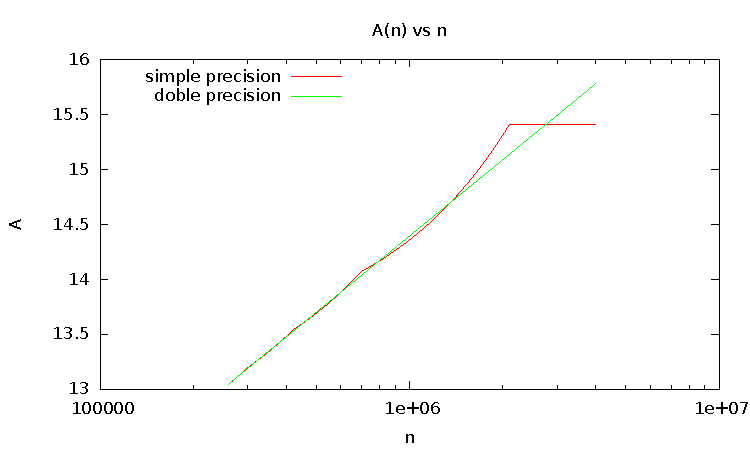
\includegraphics[width=0.8\textwidth]{./parte2/graficos/grafico_p1.pdf}
\caption{Gráfica de $A_{sp}$ y $A_{dp}$ para algunos valores de $n$. Abscisa en escala logarítmica} \label{fig_P1_1_1}
\end{center}
\end{figure}

\begin{figure} [H]
\begin{center}
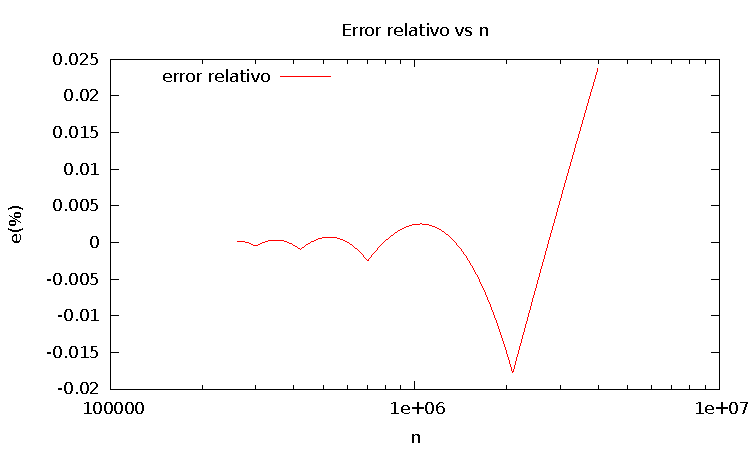
\includegraphics[width=0.8\textwidth]{./parte2/graficos/grafico_p1_error.pdf}
\caption{Error relativo $E(\%)$ de $A_{sp}$ respecto a $A_{dp}$. Abscisa en escala logarítmica} \label{fig_P1_1_2}
\end{center}
\end{figure}

%-----------------------------------------------------------------------------
%-----------------------------------------------------------------------------
%-----------------------------------------------------------------------------

\subsubsection{Ejercicio 2}
Se implementa una rutina en Fortran que permite calcular los $n+1$ valores de la serie Fibonacci
\begin{equation}
u_{n+1} = u_{n} + u_{n-1} \hspace{1cm} \mbox{tal que} \hspace{0,5cm} u_0=0 \hspace{0,1cm} ; \hspace{0,1cm} u_1=1
\end{equation}

En las Figuras \ref{fig_P1_2_1} y \ref{fig_P1_2_2} se representa los elementos de la serie. Se observa en la primera gráfica que la serie presenta un crecimiento exponencial. Para $n=46$ se presenta una inestabilidad numérica, lo cual se explica por la memoria asignada a un objeto real (Tabla  \ref{TABLA_FORTRAN}). \\

Se utiliza un real de doble precision en vez de un entero y se grafica la serie (Figura \ref{fig_P1_2_real}). Se vuelve a apreciar el comportamiento exponencial. La serie se grafica hasta que el se alcanza el tope de memoria, arrojando \textit{inf}

\begin{figure} [H]
\begin{center}
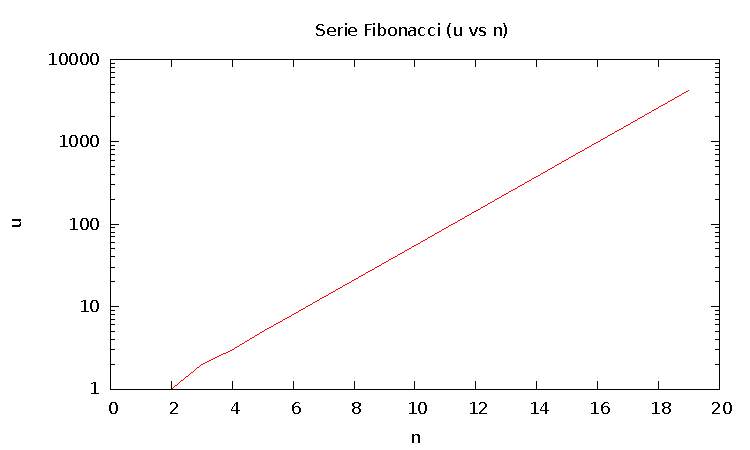
\includegraphics[width=0.8\textwidth]{./parte2/graficos/grafico_p2_1.pdf}
\caption{Gráfica de la serie Fibonacci para $n \in [0, \ldots , 20]$. Ordenanda en escala logarítmica} \label{fig_P1_2_1}
\end{center}
\end{figure}

\begin{figure} [H]
\begin{center}
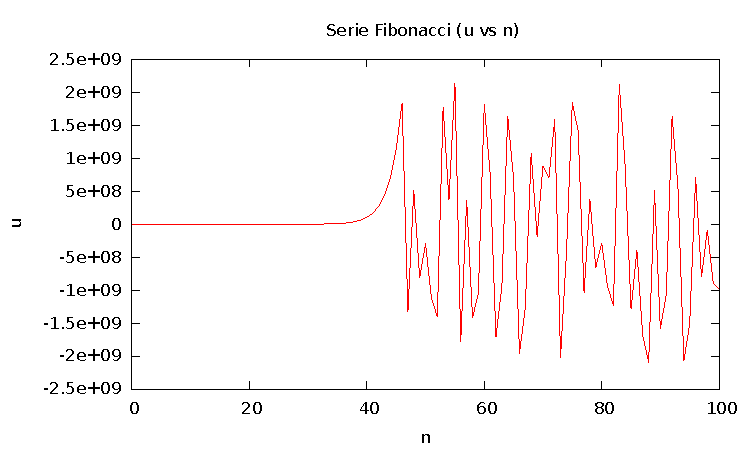
\includegraphics[width=0.8\textwidth]{./parte2/graficos/grafico_p2_2.pdf}
\caption{Gráfica de la serie Fibonacci para $n \in [0, \ldots , 100]$ definiendo $u$ como un objeto \texttt{integer}. Para $n=46$ se presenta una inestabilidad numérica: se obtiene números negativos en una serie estrictamente creciente. Ordenanda en escala logarítmica} \label{fig_P1_2_2}
\end{center}
\end{figure}

\begin{figure} [H]
\begin{center}
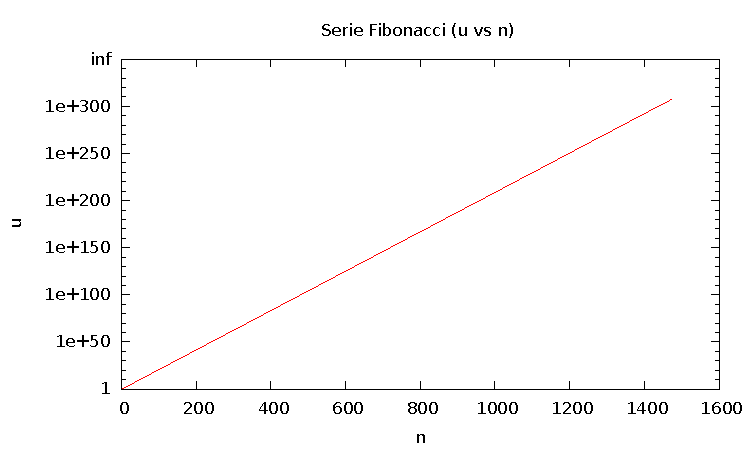
\includegraphics[width=0.8\textwidth]{./parte2/graficos/grafico_p2_real.pdf}
\caption{Gráfica de la serie Fibonacci para $n \in [0, \ldots , 1600]$ definiendo $u$ como un objeto \texttt{real} de doble precisión. El resultado crece exponencialmente hasta alcanzar el máximo de memoría permitido, arrojando \textit{inf}. Ordenanda en escala logarítmica} \label{fig_P1_2_real}
\end{center}
\end{figure}

%-----------------------------------------------------------------------------
%-----------------------------------------------------------------------------
%-----------------------------------------------------------------------------

\subsection{Ejercicio 3}

Se escribe una rutina \textit{matrix-mult} que realiza el producto entre dos matrices $\vect{A}$ y $\vect{B}$ de dimensiones $(m_a,n_a)$ y $(m_b,n_b)$ respectivamente. El algoritmo implementado es el siguiente:
\begin{enumerate}
\item Se ingresan los valores de las matrices $\vect{A}_{n_a,m_a}$ y $\vect{B}_{n_b,m_b}$.
\item Se verifica la dimensión entre $\vect{A}$ y $\vect{B}$. Si $m_a \neq n_b$ entonces $l=1$ y se sale de la subrutina. En el caso contrario, las dimensiones son consistente con la multiplicación matricial, $l=0$, y se pasa al siguiente paso ($l$: indicador del error)
\item Se define el tamaño y se asigna la memoria para arreglo $C_{n_a,m_b}$
\item Se realiza la multiplicación matricial entre $\vect{A}$ y $\vect{B}$. Se asigna a la matriz $\vect{C}$
\item Salida de la subrutina $\vect{C_}{n_a,m_b}$ y $l$
\end{enumerate}
En la Figura \ref{fig_P1_3} se expone un diagrama de flujo que explica la subrutina

\begin{figure} [H]
\begin{center}
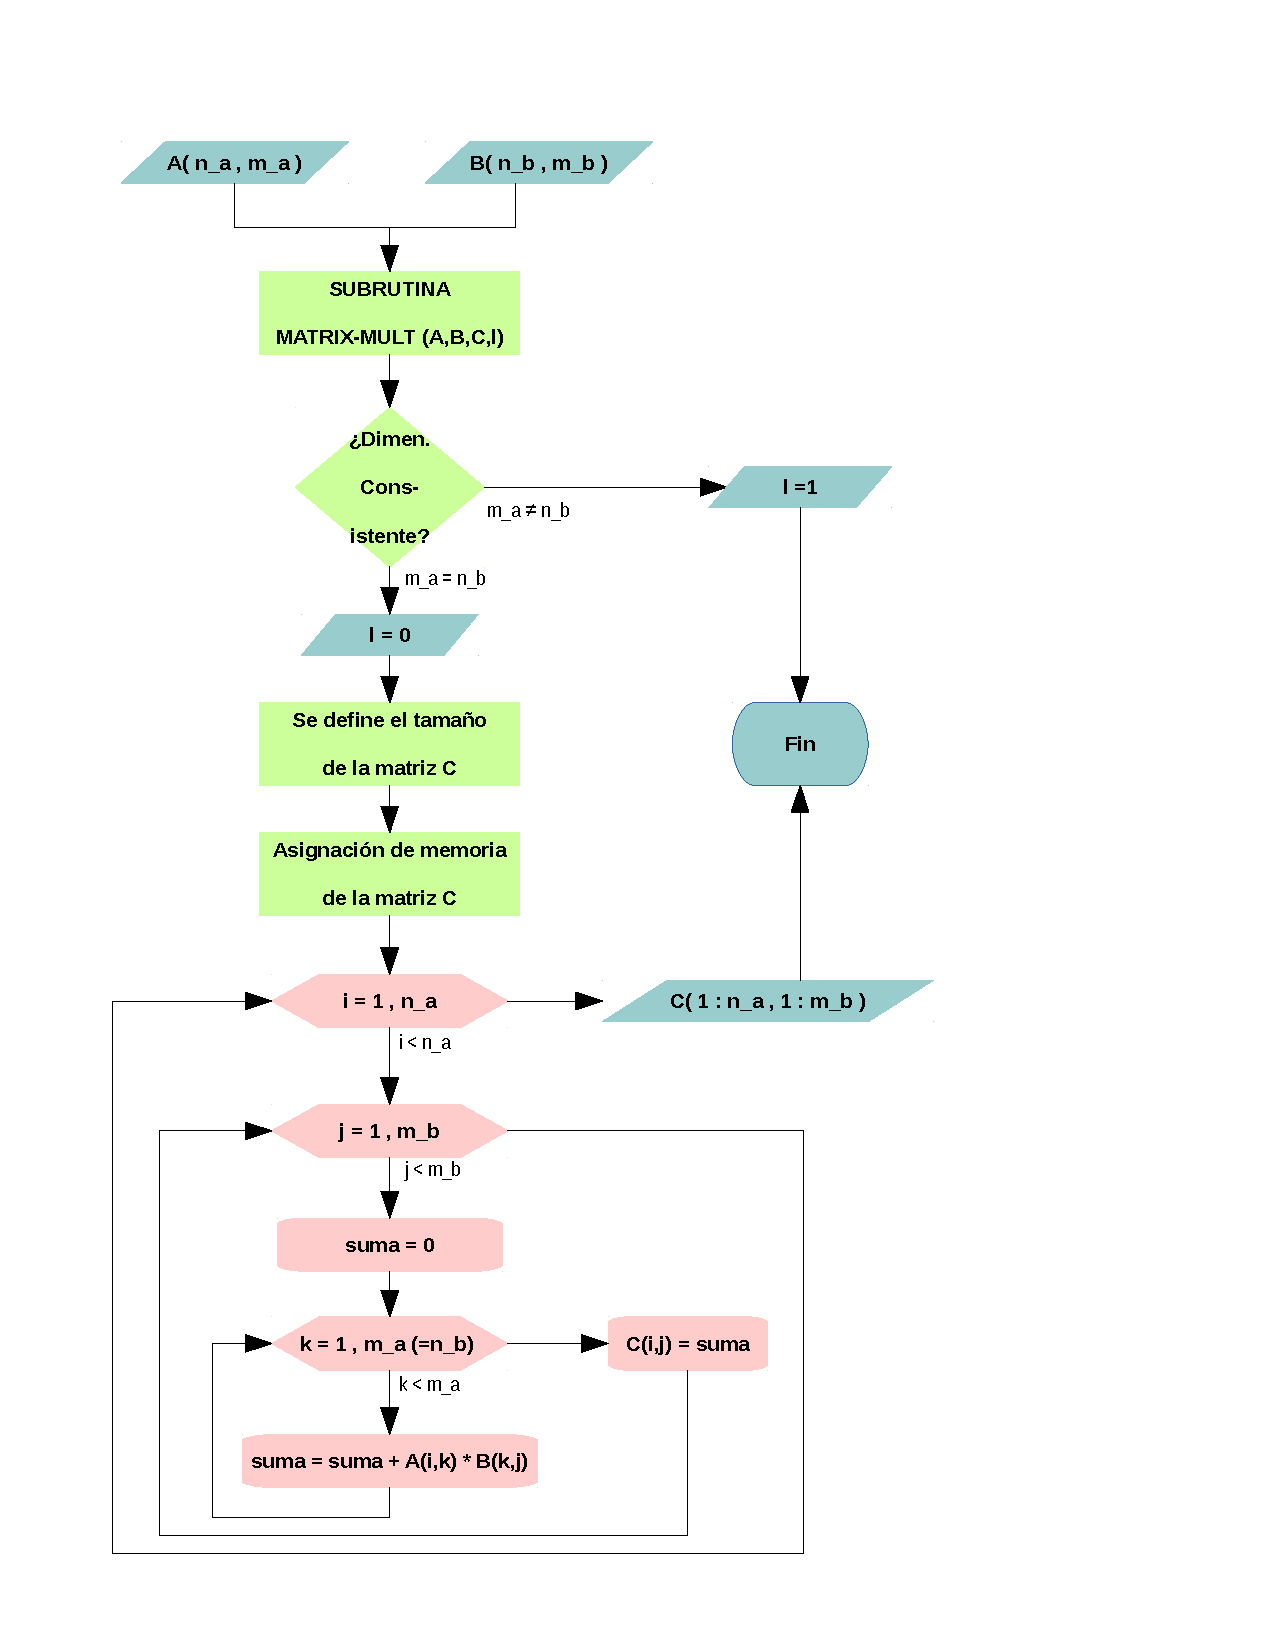
\includegraphics[width=0.9\textwidth]{./parte2/graficos/diagrama_de_flujo.pdf}
\caption{Diagrama de flujo de la subrutina \textit{matrix-mult}. Variables de entrada: Matrices $\vect{A}_{n_a,m_a}$ y $\vect{B}_{n_b,m_b}$. Variables de salida: Matriz $\vect{C}_{n_a,m_b}$ y el indicador de error $l$} \label{fig_P1_3}
\end{center}
\end{figure}
